\section{Patient History Graph Implementation}
\label{sec:graph_logic}

A core distinguishing feature of the CFI-Care backend is the Patient History
Graph, which visualizes a patient's medical journey as a Directed Acyclic Graph
(DAG). Unlike standard FHIR lists, which present data linearly, this graph
models causal and temporal relationships between medical events. This
representation provides clinicians with a sophisticated tool for understanding
the evolution of a patient's condition, particularly in complex cases involving
multiple concurrent diagnoses or extended treatment histories.

\subsection{Motivation: Beyond Linear Medical Records}
\label{subsec:graph_motivation}

Traditional Electronic Health Records (\ac{EHR}s) typically present patient
data as chronologically ordered events: a consultation on January 1st, a lab
test on January 3rd, a prescription on January 5th, and so forth. While this
linear representation is straightforward to implement and understand, it
obscures the causal relationships that are essential to clinical reasoning.
Consider a patient with Type 2 Diabetes presenting with hypertension and
elevated cholesterol levels. In a linear record, these appear as separate
events without explicit connection. However, a clinician recognizes that these
conditions are causally related---elevated cholesterol and hypertension may be
comorbidities stemming from the underlying metabolic dysfunction of diabetes.

The Patient History Graph addresses this limitation by explicitly modeling
causality and temporal dependencies. Each medical event is represented as a
node in the graph, and directed edges represent causal or temporal
relationships. This graphical representation allows clinicians to trace the
progression of a specific condition across multiple encounters and
interventions, identify temporal clusters of related events that may indicate
disease progression or treatment response, visualize the impact of therapeutic
interventions on subsequent clinical outcomes, and differentiate between
independent medical episodes and related sequences of events. By making these
relationships explicit, the graph transforms raw temporal sequences into
clinically meaningful narratives that support more effective decision-making.

\begin{figure}[H]
    \centering
    \fbox{\begin{minipage}{\dimexpr\textwidth-2\fboxsep-2\fboxrule\relax}
            \centering
            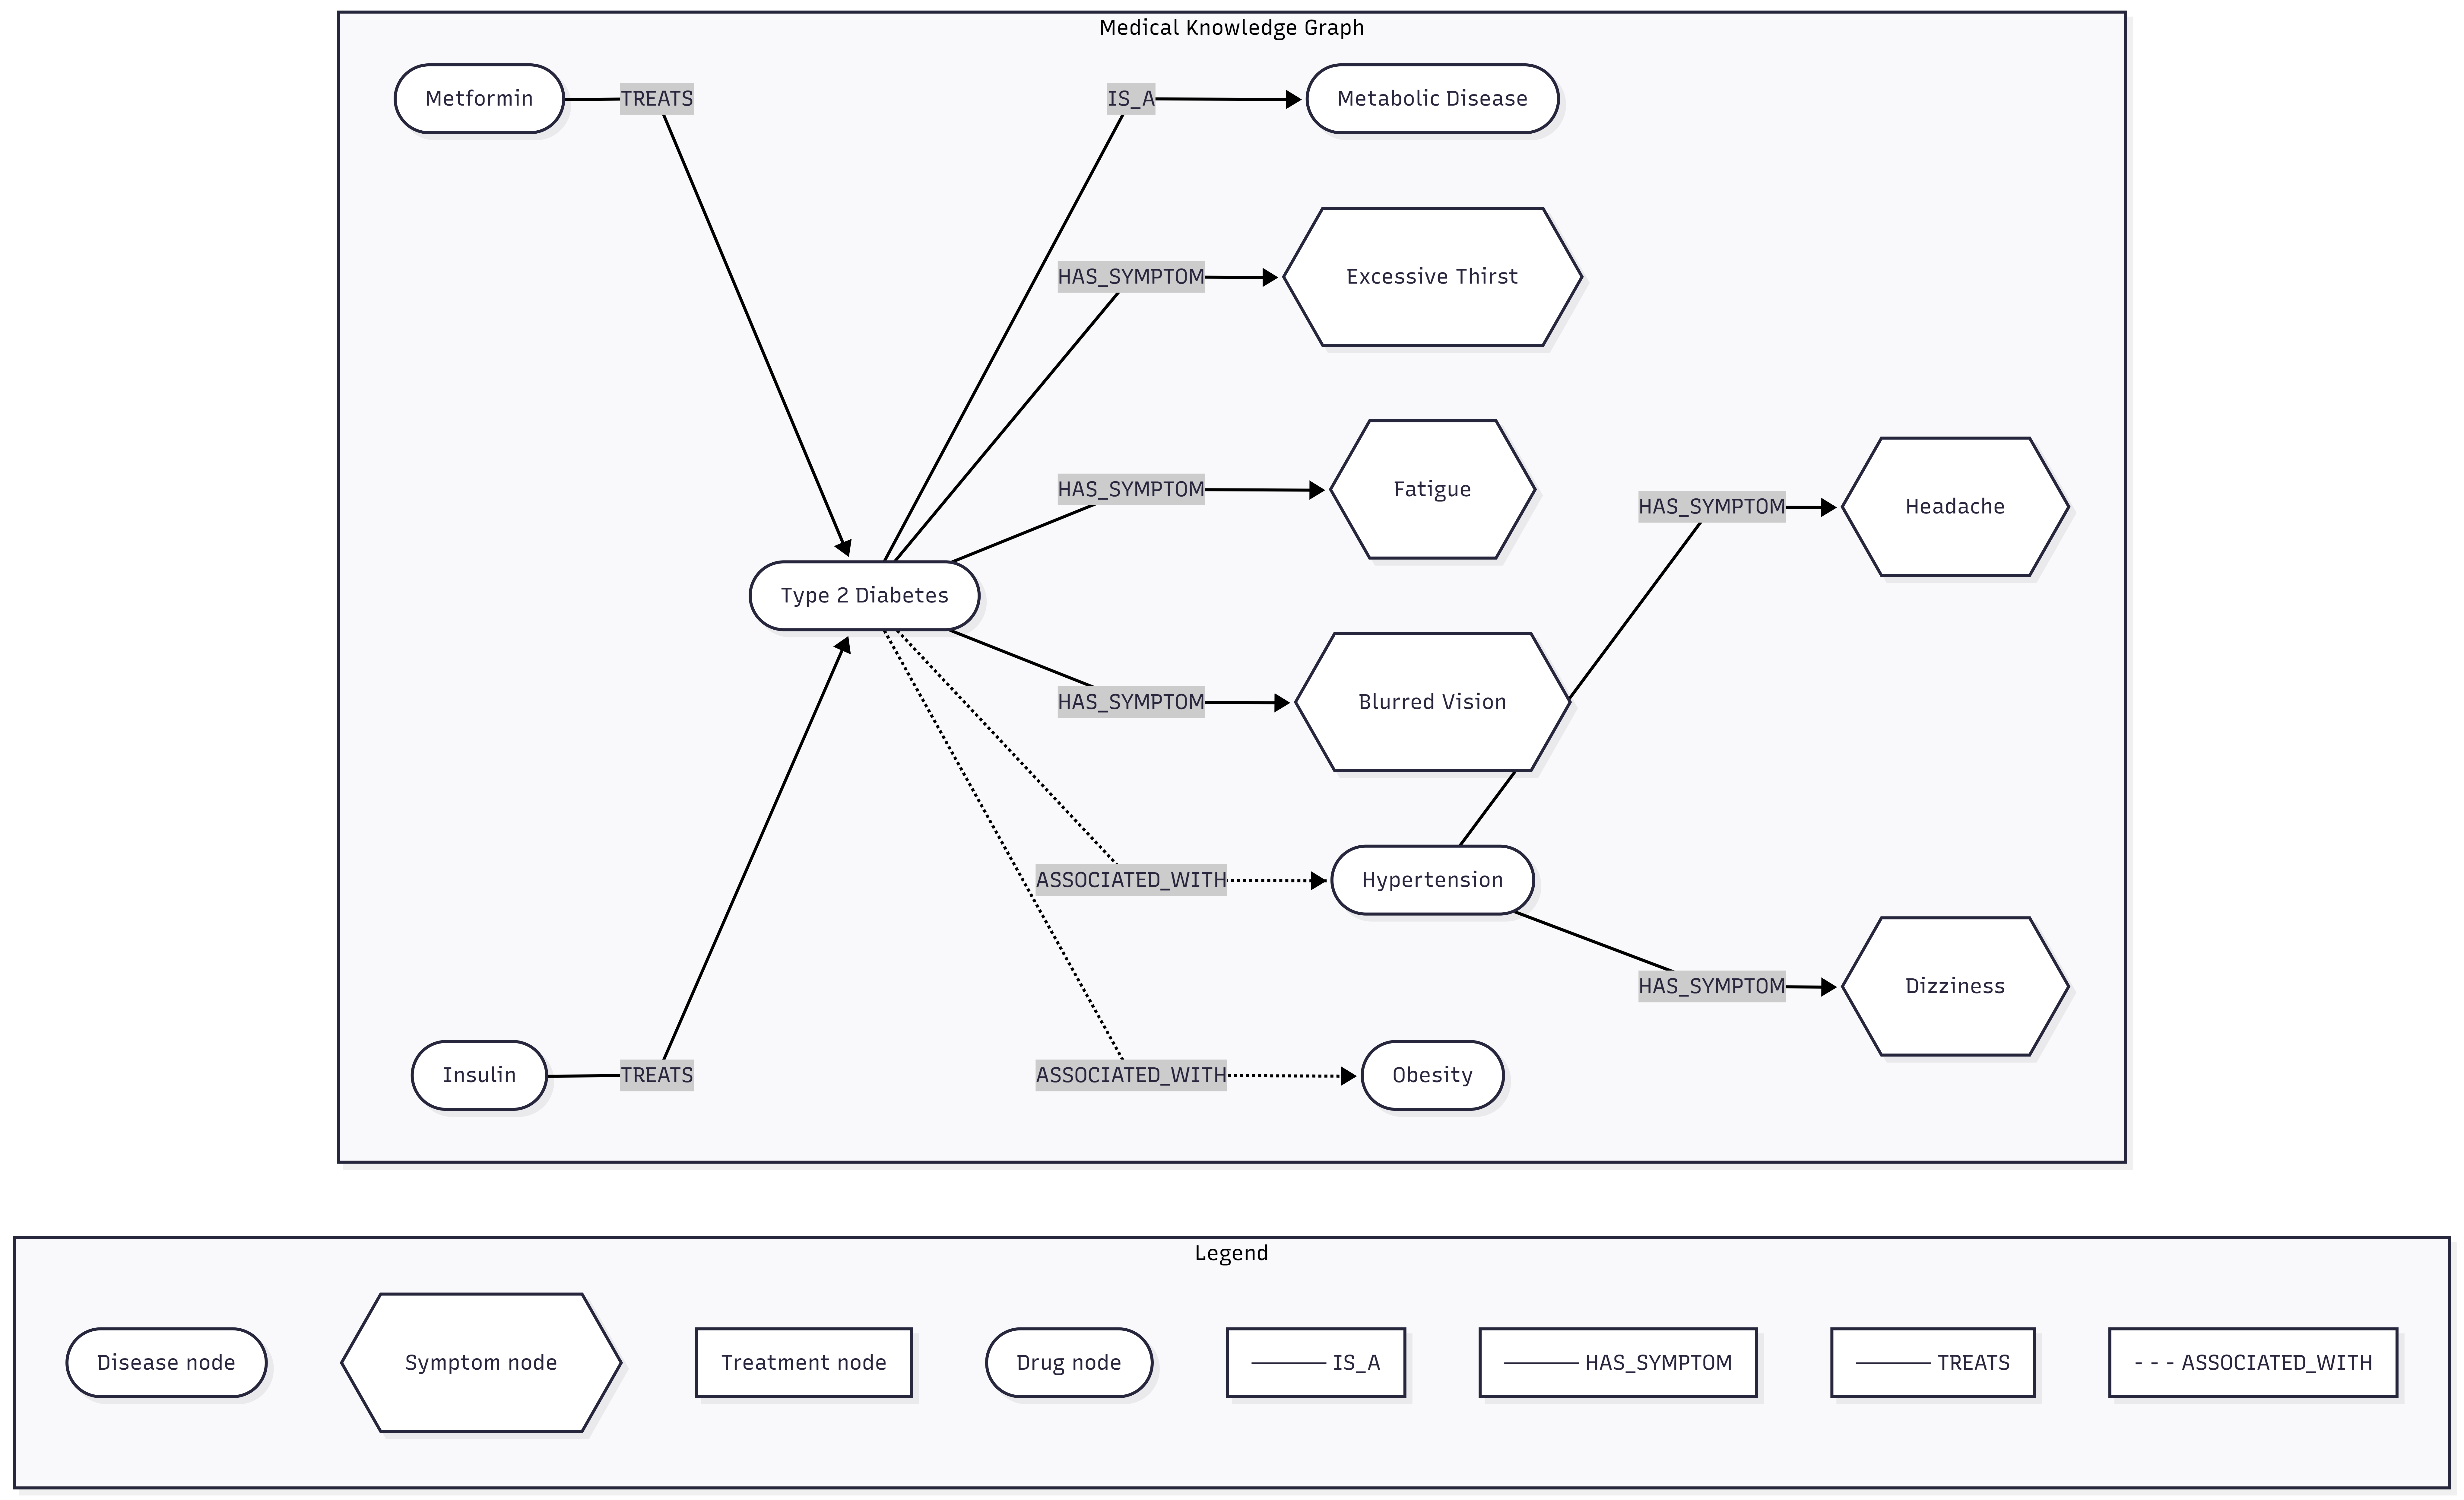
\includegraphics[width=0.9\linewidth]{Backend/Images/graphDiagram.png}
            % \vspace{6.5cm}
            % \textbf{FIGURE INSTRUCTION:} \\
            % \textit{Create a Patient History Graph Visualization Example.} \\
            % \textbf{Content:} Create an actual directed acyclic graph (DAG) showing a realistic patient journey. \\
            % \textbf{Example Scenario - Diabetes Patient with Concurrent Hypertension:} \\
            % \textbf{Branch 1 (Diabetes - Main timeline):} \\
            % Node 1: Consultation (Jan 1, 2025) - "Patient presents with increased thirst, fatigue" \\
            % ↓ (causal edge, confidence: 0.9) \\
            % Node 2: Lab Result (Jan 1, 2025) - "HbA1c: 8.2\%, Fasting Glucose: 180 mg/dL" \\
            % ↓ (causal edge, confidence: 0.95) \\
            % Node 3: Diagnosis (Jan 2, 2025) - "Type 2 Diabetes Mellitus (ICD-10: E11)" \\
            % ↓ (causal edge, confidence: 0.98) \\
            % Node 4: Prescription (Jan 2, 2025) - "Metformin 500mg BID" \\
            % ↓ (temporal edge, confidence: 0.7) \\
            % Node 5: Lab Result (Apr 1, 2025) - "HbA1c: 6.8\% (improved)" \\
            % \textbf{Branch 2 (Hypertension - Concurrent):} \\
            % Node 6: Vital (Feb 15, 2025) - "BP: 145/95 mmHg" [NEW HEAD NODE] \\
            % ↓ (temporal edge, confidence: 0.6) \\
            % Node 7: Diagnosis (Feb 15, 2025) - "Essential Hypertension (ICD-10: I10)" \\
            % ↓ (causal edge, confidence: 0.9) \\
            % Node 8: Prescription (Feb 16, 2025) - "Lisinopril 10mg daily" \\
            % \textbf{Visual Requirements:} \\
            % - Use different shapes: Hexagon (Consultation), Circle (Lab/Vital), Diamond (Diagnosis), Rectangle (Prescription) \\
            % - Color code by branch: Blue for diabetes, Green for hypertension \\
            % - Edge thickness by confidence: Thick (>0.8), Medium (0.6-0.8), Thin (<0.6) \\
            % - Edge labels: relationship type (causal/temporal/associative) \\
            % - Show dates on each node \\
            % - Clearly separate the two branches visually (side-by-side layout) \\
            % \textbf{Recommended Tool:} D3.js export, Graphviz, yEd, or Draw.io with graph layout.
        \end{minipage}}
    \caption{Example Patient History Graph showing a diabetes patient with concurrent hypertension, demonstrating temporal branching and multiple relationship types.}
    \label{fig:patient_history_graph_example}
\end{figure}

\subsection{Graph Data Model}
\label{subsec:graph_model}

The Patient History Graph is built upon a relational foundation with two
primary tables: \texttt{encounter\_nodes} and \texttt{node\_relations}.

\subsubsection{Node Representation}
Each node in the graph represents a distinct clinical event or observation. The
system supports nine node types. \texttt{Consultation} represents a clinical
encounter between patient and clinician. \texttt{Diagnosis} denotes a confirmed
medical condition recorded during or after a consultation. \texttt{Prescription}
indicates a medication prescribed to address a specific condition.
\texttt{LabResult} captures laboratory or diagnostic test results. \texttt{Vital}
encompasses blood pressure, temperature, and other vital signs. \texttt{Symptom}
represents patient-reported subjective findings. \texttt{FollowUp} schedules a
future clinical visit; creating a FollowUp node with a future \texttt{event\_date}
automatically triggers FHIR Appointment provisioning, described in
Section~\ref{subsec:followup_nodes}. \texttt{AISuggestion} captures
AI-generated clinical recommendations produced by the MedGemma reasoning engine.
\texttt{Allergy} records patient allergy information linked to a corresponding
FHIR AllergyIntolerance resource.

Each node in the \texttt{encounter\_nodes} table stores the following metadata:
the \texttt{patient\_id} and \texttt{practitioner\_id} identifying the involved
parties; an \texttt{fhir\_resource\_id} linking back to the source FHIR resource
for full data provenance; the node's \texttt{category} and \texttt{event\_date};
a \texttt{branch\_id} referencing the root node of the branch this node belongs
to (null for root/head nodes); a \texttt{branch\_state} attribute
(\texttt{in\_progress} or \texttt{completed}) indicating the clinical resolution
of the episode; boolean flags \texttt{is\_diagnosis} and
\texttt{is\_manual\_branch} distinguishing system-detected diagnostic branches
from manually initiated ones; a \texttt{related\_resource\_ids} JSON array for
auxiliary FHIR references; and an \texttt{is\_deleted} soft-delete flag that
preserves historical integrity while hiding logically removed records.

A fundamental design principle of the Patient History Graph is immutability:
nodes are never physically deleted. The \texttt{is\_deleted} flag and a
corresponding \texttt{deleted\_at} timestamp are used instead, ensuring that the
graph preserves a complete and auditable record of every recorded event.

\subsubsection{Edge Representation}
Edges in the graph represent directed relationships between clinical events. An
edge from node $A$ to node $B$ indicates that event $A$ preceded and influenced
event $B$ in some clinically meaningful way. The \texttt{node\_relations} table
stores each edge as a \texttt{source\_node\_id}/\texttt{target\_node\_id} pair
alongside a \texttt{relationship\_type} classifying the semantic nature of the
connection. The table also carries \texttt{is\_deleted} and \texttt{deleted\_at}
fields, applying the same soft-delete policy as nodes to maintain a
non-destructive audit trail. The seven relationship types are described in
Section~\ref{subsec:relationship_types}.

% \subsection{Graph Construction Algorithm}
% \label{subsec:graph_construction}

% The graph construction logic is encapsulated within the
% \texttt{historyGraphService}, a core backend service invoked whenever a new
% medical event is recorded. The algorithm operates in several stages:

% \subsubsection{Stage 1: Node Creation}
% When a new clinical event is received from the FHIR server (such as a new
% prescription, lab result, or consultation record), the system creates a
% corresponding node in the \texttt{encounter\_nodes} database table. This node
% captures essential event information: the patient to which the event belongs,
% the clinical category of the event (Consultation, Diagnosis, Prescription,
% etc.), the timestamp indicating when the event occurred, a reference ID linking
% back to the source FHIR resource for data provenance, and structured clinical
% details extracted from the FHIR resource including diagnosis codes, medication
% specifications, laboratory values, and other relevant clinical parameters.

% \subsubsection{Stage 2: Temporal Scanning and Parent Identification}
% After node creation, the algorithm performs a critical temporal backward scan
% of all existing nodes for the patient to identify potential parent nodes. This
% scan is bounded by three sets of clinical rules that determine what types of
% events can meaningfully be causally related. First, event type rules enforce
% domain-specific constraints: for instance, a Prescription node can only have a
% Consultation, Diagnosis, or another Prescription as a parent, while a
% Consultation cannot have a Prescription as a parent. These rules prevent
% semantically meaningless relationships from being created. Second, temporal
% window constraints ensure that relationships are only established between
% events within a clinically relevant time window. A prescription issued more
% than six months after a consultation is statistically unlikely to be causally
% related unless additional context suggests otherwise. Third, specificity
% matching ensures that the algorithm correctly associates events with their most
% clinically relevant predecessors. For example, a prescription for metformin
% (used in diabetes management) is linked to the most recent Diabetes diagnosis
% rather than to an unrelated hypertension diagnosis, even if both diagnoses
% exist in the patient's history.

% The algorithm identifies the most recent "eligible" parent node based on these
% constraints. In cases where multiple candidates exist with similar temporal
% proximity, the system selects the most clinically specific match, prioritizing
% condition-specific diagnoses over generic symptoms or vice versa depending on
% the event context.

% \subsubsection{Stage 3: Edge Creation}
% Once a parent node is identified, a directed edge is created from parent to
% child in the \texttt{node\_relations} table. The edge stores metadata including
% the relationship type (causal, temporal, or associative) and a confidence score
% indicating the algorithm's certainty in the relationship.

% \subsubsection{Algorithm Pseudocode}
% The following pseudocode formalizes the algorithm:

% \begin{verbatim}
% function constructGraphNode(newEvent, patientId):
%     // Stage 1: Create node
%     node = createNode(newEvent, patientId)

%     // Stage 2: Scan for parents
%     existingNodes = queryNodesByPatient(patientId)
%     candidateParents = []

%     for existingNode in existingNodes:
%         if isValidRelationship(newEvent.type, existingNode.type):
%             if isWithinTemporalWindow(newEvent, existingNode):
%                 if matchesClinicalContext(newEvent, existingNode):
%                     candidateParents.add(existingNode)

%     // Stage 3: Select and link parent
%     if candidateParents is not empty:
%         parentNode = selectMostRelevantParent(candidateParents)
%         createRelation(parentNode, node)
%     end if

%     // Invalidate cache
%     invalidateGraphCache(patientId)

%     return node
% end function
% \end{verbatim}

\subsection{Temporal Branching and Concurrent Episodes}
\label{subsec:temporal_branching}

Real-world patient histories are rarely linear. A patient may have multiple
concurrent health issues being managed in parallel. For example, a patient may
simultaneously receive treatment for diabetes, hypertension, and arthritis. In
a traditional linear \ac{EHR}, this complexity is flattened; all events appear
chronologically without indication of which episode they belong to.

The CFI-Care graph model handles this through an explicit branching mechanism:

\subsubsection{Head Node Concept}
A "Head Node" is a node with no outgoing edges to other nodes in the current
timestamp window. When a new clinical event arrives that does not fit within
any existing causal chain (i.e., no valid parent is found), the system creates
a new Head Node, effectively initiating a new branch in the history graph.

For example, consider a patient's history:
\begin{enumerate}
    \item Consultation for chest pain (2025-01-01)
    \item EKG test (2025-01-01)
    \item Cardiology referral (2025-01-02)
    \item New consultation for joint pain (2025-02-15) — \textbf{New Branch}
    \item X-ray of knee (2025-02-15)
    \item Rheumatology referral (2025-02-16)
\end{enumerate}

The system recognizes that the joint pain consultation on 2025-02-15 cannot be
causally linked to the earlier cardiology events (temporal gap exceeds
threshold, clinical context is unrelated). Therefore, it creates a new Head
Node for the rheumatology branch, allowing clinicians to visually separate the
two episodes.

\subsubsection{Visual Implications}
From a visualization perspective, branching creates a multi-root forest
structure (multiple separate trees within the graph). The frontend rendering
engine positions these branches side-by-side or in hierarchical layout,
enabling clinicians to track multiple concurrent conditions without visual
clutter or confusion.

\subsubsection{Branch State Lifecycle}
Each branch carries an explicit \texttt{branch\_state} attribute that tracks
the clinical resolution of its episode. A branch is initialized in the
\texttt{in\_progress} state when its head node is created, indicating an active
or unresolved clinical episode. The state transitions to \texttt{completed} when
a clinician closes the branch---typically following a discharge, condition
resolution, or explicit closure of the clinical episode.

This lifecycle gives clinicians an immediate visual indicator of which medical
episodes are ongoing and which have been resolved, and the frontend exposes
branch-level filtering on this attribute so that only active conditions are
surfaced during an acute consultation while the full historical record remains
accessible.

\subsubsection{Clinical Advantages}
Explicit branching provides significant clinical benefits that improve the
utility of the Patient History Graph. Clinicians immediately recognize which
events belong to which condition through visual separation, substantially
reducing cognitive load compared to linearly ordered records. The system can
provide condition-specific recommendations by analyzing the isolated branch
rather than considering the entire patient history, enabling more targeted and
relevant clinical decision support. Additionally, each branch can be summarized
independently for specialist-to-specialist referrals, allowing specialists to
focus on the specific problem domain without irrelevant context from other
concurrent conditions.

\subsection{Relationship Classification}
\label{subsec:relationship_types}

Not all edges in the Patient History Graph carry the same semantic weight or
clinical significance. The system implements seven distinct relationship types,
each persisted in the \texttt{relationship\_type} column of
\texttt{node\_relations}:

\begin{itemize}
    \item \textbf{\texttt{causes}}: Node $A$ directly caused or necessitated
    Node $B$. Example: a Diabetes Diagnosis causes a Metformin Prescription.
    This is the highest-confidence relationship type.

    \item \textbf{\texttt{derives\_from}}: Node $B$ is a clinical derivation of
    Node $A$---for instance, a Diagnosis derived from a LabResult that confirmed
    the condition.

    \item \textbf{\texttt{follows}}: Node $B$ occurred sequentially after Node
    $A$ within the same clinical episode without an explicit causal link---for
    example, a Blood Pressure Vital reading taken during the same consultation as
    a preceding Symptom.

    \item \textbf{\texttt{documents}}: Node $B$ formally documents or records
    Node $A$---typically used when a Consultation node documents a
    patient-reported Symptom.

    \item \textbf{\texttt{association}}: Node $A$ and Node $B$ share clinical
    context without direct causation---such as concurrent comorbidities stemming
    from the same underlying metabolic dysfunction.

    \item \textbf{\texttt{references}}: Node $B$ cites or references Node $A$
    without implying a causal or temporal sequence, used for cross-episode
    clinical annotations.

    \item \textbf{\texttt{contains}}: Node $A$ hierarchically contains Node
    $B$---for example, an Encounter node containing a set of constituent
    Observations or Prescriptions issued during that encounter.
\end{itemize}

Each relationship also stores a confidence score from 0.0 to 1.0 generated by
the construction algorithm. High-confidence relationships (score $>$ 0.8) are
displayed prominently in the visualization, while lower-confidence edges are
rendered with reduced visual emphasis or as optional links the clinician can
explore on demand.

\subsection{Handling Edge Cases}
\label{subsec:edge_cases}

The Patient History Graph implementation must gracefully handle several
challenging scenarios that arise in real-world clinical practice. Retroactive
diagnosis occurs when a patient receives a diagnosis that applies to earlier
symptoms after those symptoms have already been recorded. For example, a
patient might experience chest pain on January 1st and only receive a diagnosis
of coronary artery disease on March 1st. The algorithm detects this temporal
mismatch and retroactively relinks the symptom node to the new diagnosis,
maintaining causal clarity and preventing the false impression that the symptom
was unexplained.

Conflicting information presents another challenge. When new FHIR data
contradicts previously recorded information---such as a diagnosis being
changed, retracted, or corrected---the system must handle this gracefully.
Rather than deleting nodes (which would violate the immutability principle and
destroy the audit trail), the system creates a new node representing the
correction and links it appropriately to existing nodes. This approach
preserves the complete historical record while accurately reflecting the
current clinical understanding.

Circular references represent a potential structural problem. Although directed
acyclic graphs (DAGs) cannot, by definition, contain cycles, the algorithm must
validate that no accidental cycles are introduced during edge creation. This
validation is enforced through topological sorting checks performed before
persisting relationships to the database, preventing data consistency issues
that could arise from cycles.

\subsection{FollowUp Nodes and Automated Appointment Scheduling}
\label{subsec:followup_nodes}

A specialized node type, \texttt{FollowUp}, integrates the graph layer directly
with the FHIR scheduling layer. When a clinician records a follow-up visit with
a future \texttt{event\_date}, the \texttt{historyGraphService} automatically
provisions a corresponding FHIR \texttt{Appointment} resource. The appointment
is created with a status of \texttt{booked} and a default duration of 30
minutes, with participant entries automatically populated for both the patient
and the recording practitioner.

This automation eliminates the manual step of separately navigating to a
scheduling module after completing a clinical encounter. The \texttt{FollowUp}
node is linked to its parent encounter node via a \texttt{follows} or
\texttt{causes} relationship, preserving the clinical chain of reasoning that
motivated the appointment within the graph. Should the appointment be cancelled
or rescheduled, the corresponding graph node is soft-deleted
(\texttt{is\_deleted = true}), maintaining an auditable record of the original
scheduling intent without corrupting the graph topology.

\subsection{Query Patterns and Optimization}
\label{subsec:graph_queries}

The frontend visualization layer requires efficient access to the graph
structure through several common query patterns, each optimized for specific
clinical use cases. Full Graph Retrieval fetches all nodes and edges for a
patient, which is necessary during the initial page load when clinicians first
view a patient's complete medical history. This operation is optimized through
caching strategies discussed in Section \ref{sec:backend_optimization}.
Ancestor Traversal answers questions such as "What led to this prescription?"
by fetching all ancestor nodes of a specific event. This pattern is implemented
via recursive queries that are bounded by depth to prevent unbounded
traversals. Branch Isolation allows clinicians to focus on specific medical
episodes, such as "Show only cardiology-related events," by fetching all nodes
within a specific branch. This operation uses topological partitioning to
efficiently isolate branches without scanning the entire graph. Temporal Range
Queries retrieve nodes within a specific date range, enabling clinicians to
analyze disease progression over a specific time period. These queries leverage
indexed timestamp columns to achieve O(log n) lookup time complexity, ensuring
responsiveness even for patients with extensive histories.

